%!TEX root = ./thesis-main.tex
\chapter{Conclusione}
La totalità delle considerazioni e delle tecniche di sviluppo affrontate in questo documento ha portato alla creazione di una interfaccia web capace di rappresentare correttamente l'ambiente delle simulazioni di Alchemist, facendo uso delle \ac{API} GraphQL e utilizzando come linguaggio di sviluppo KotlinJS. Questo ha permesso di usare tecnologie coerenti alla \textit{code-base} esistente, evitando di usare stack tecnologici incompatibili che ne avrebbero potuto complicare l'integrazione. Il lavoro compiuto ha portato alla creazione di un prodotto allineato con le esigenze e gli obiettivi del progetto. 
Si è fatto impiego di strumenti, tra cui librerie e framework popolari, che godono di un continuo supporto in termini di aggiornamenti e correzioni da parte di una community attiva. L'utilizzo di tali risorse ha agevolato il processo di sviluppo e fornito una solida base su cui costruire e ampliare il prodotto.
È importante far notare come il risultato finale, allo stato attuale, non rappresenta il completo funzionamento del sistema, principalmente a causa della stretta dipendenza dalle \ac{API} fornite. Questa dipendenza limita la capacità di rappresentare tutte le potenzialità del sistema. Inoltre, per rispettare i requisiti iniziali nelle tempistiche a disposizione, si è dovuto utilizzare solo un sottoinsieme delle possibili interrogazioni, il che, di conseguenza, risulta in rappresentazioni limitate. In ogni caso, questo progetto fornisce un punto di partenza per l'espansione delle funzionalità e il miglioramento delle rappresentazioni future. Alcune di queste sono esplorate nella sezione successiva.

A titolo di esempio, vengono presentati due casi illustrativi.

Nella figura \cref{fig:protelis-example} si osserva l'interfaccia grafica che mostra una simulazione in esecuzione con l'incarnation protelis\footnote{\url{https://alchemistsimulator.github.io/reference/yaml/}}. In questa configurazione, gli agenti cognitivi sono incaricati di evitare una zona pericolosa mentre si dirigono verso un obiettivo. Gli agenti si possono spingere tra di loro, creando variazioni uniche ad ogni esecuzione.
\begin{figure}
	\centering
	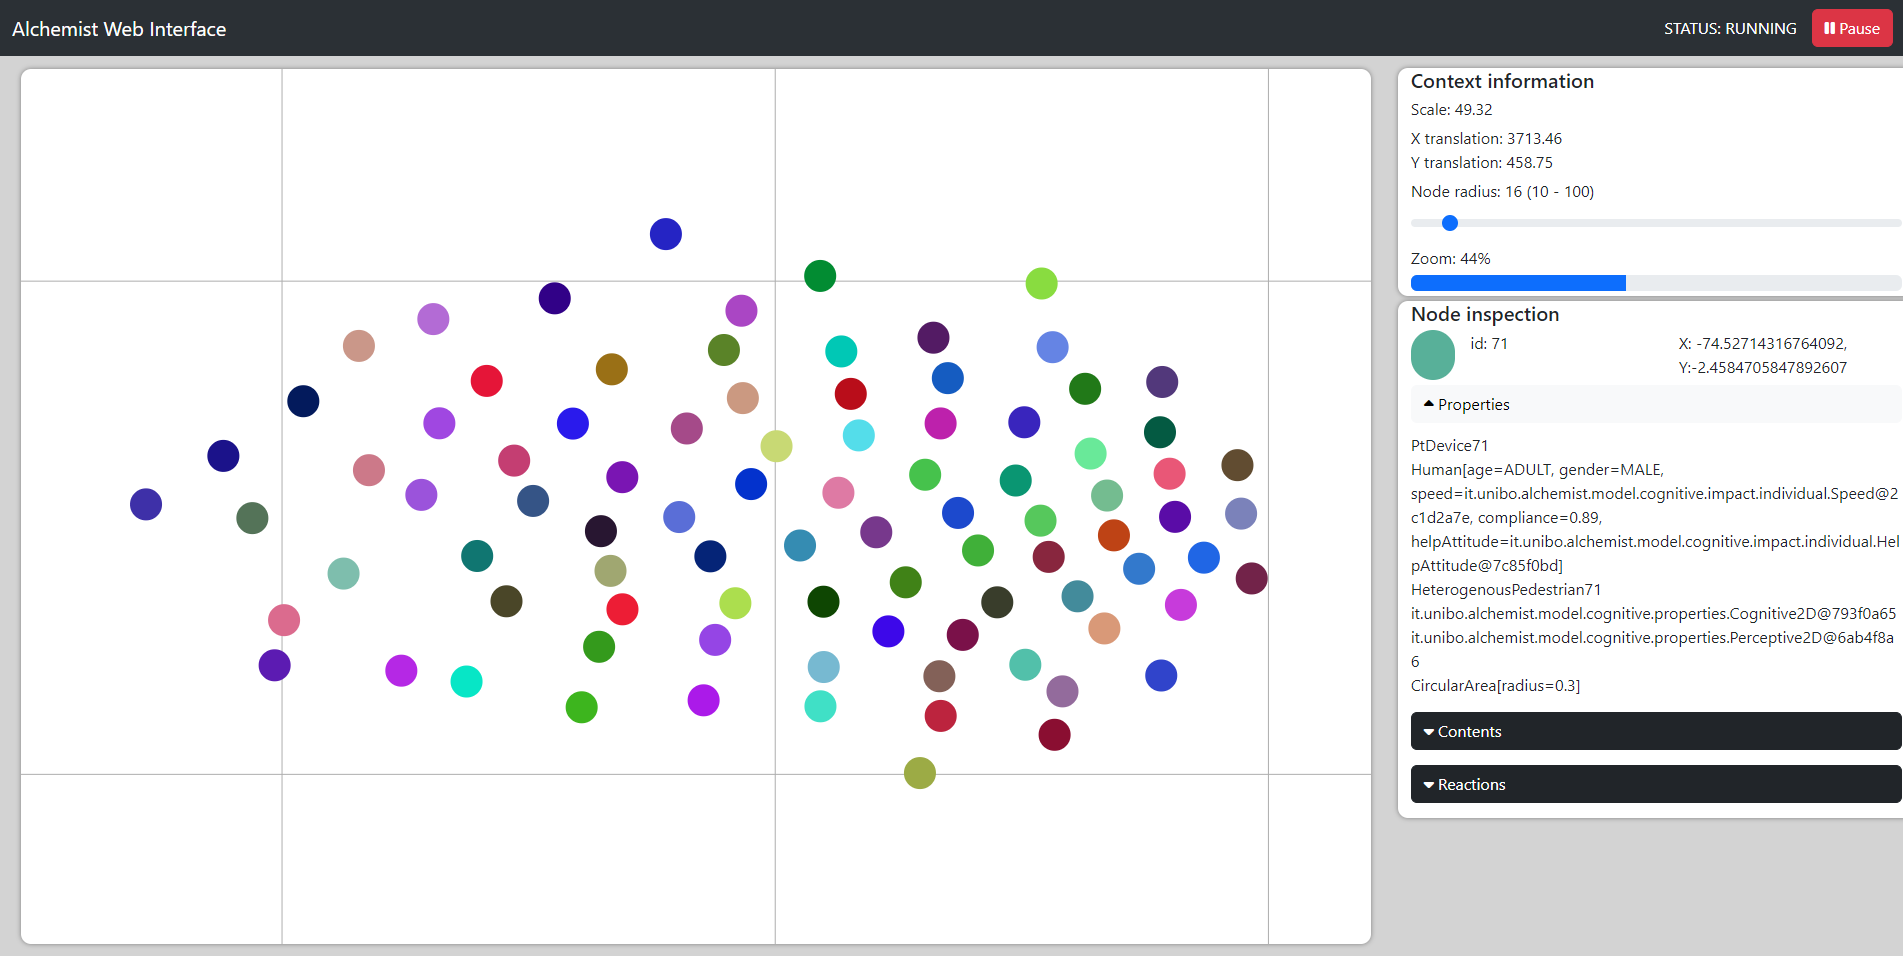
\includegraphics[scale=0.22]{imgs/screens/example_protelis.png}
	\caption{Esempio di simulazione tramite l'\textit{incarnation} protelis}
	\label{fig:protelis-example}
\end{figure}
\begin{figure}
	\centering
	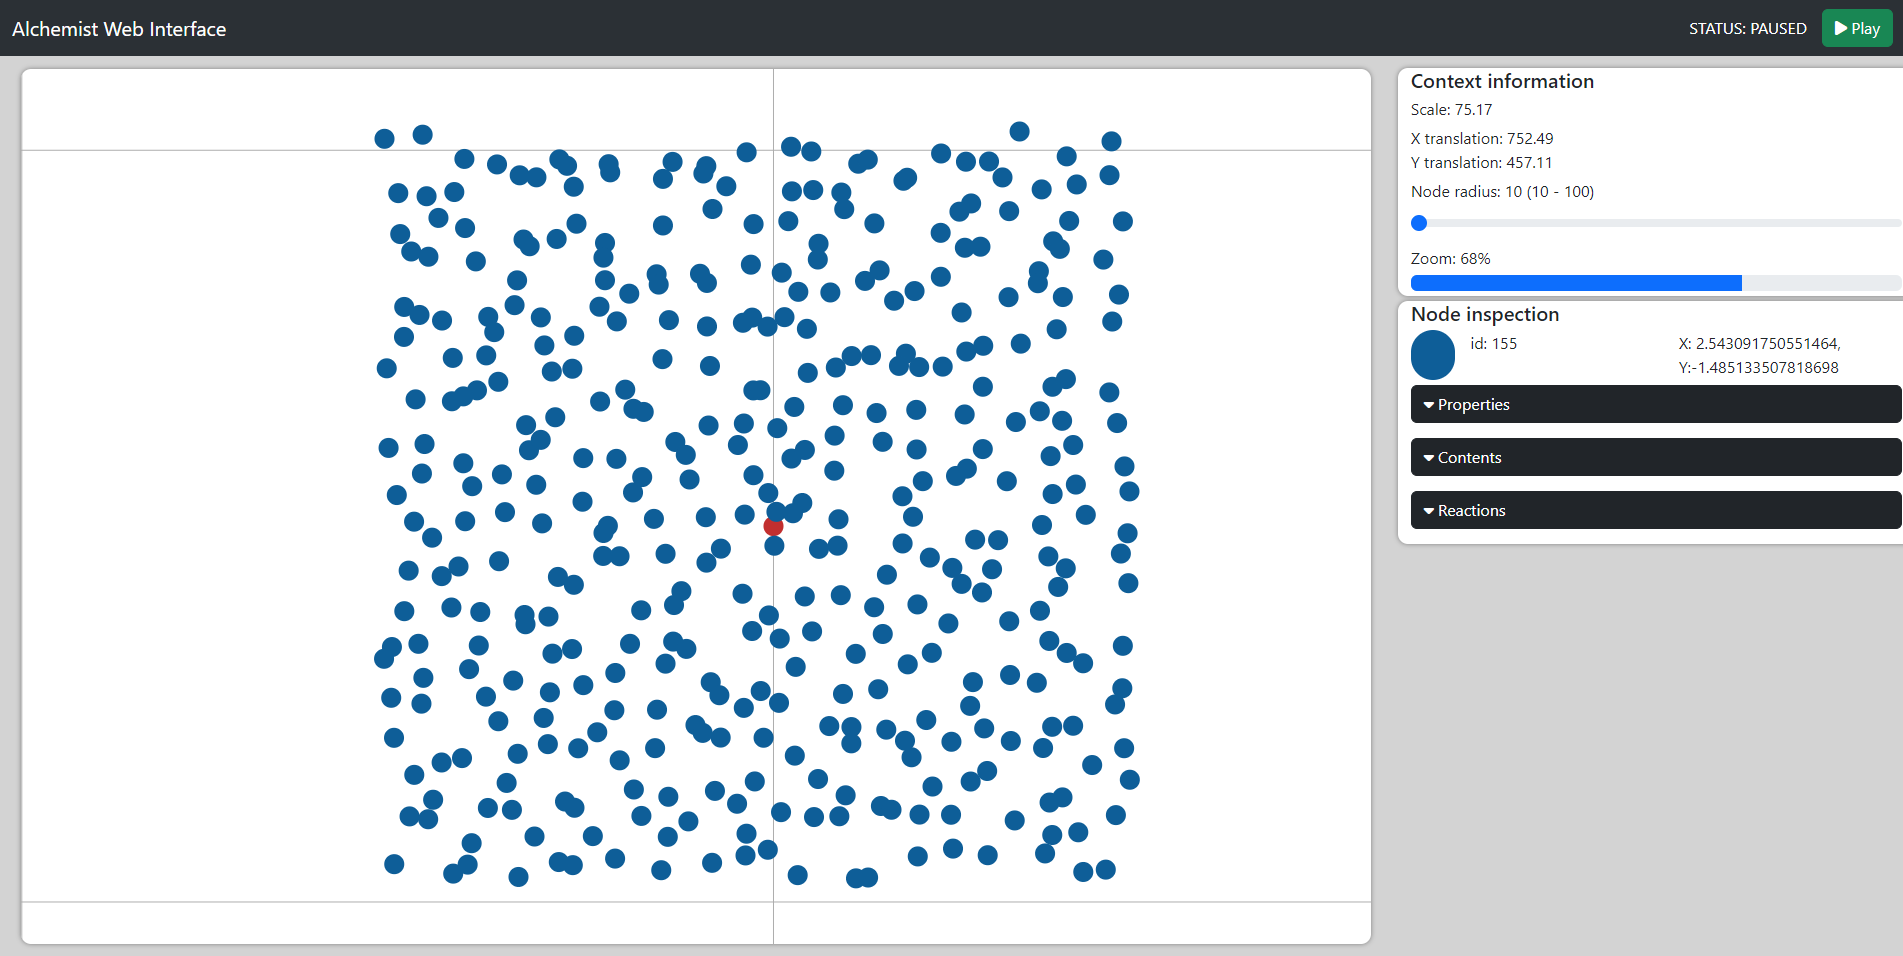
\includegraphics[scale=0.22]{imgs/screens/example_sapere.png}
	\caption{Esempio di simulazione tramite l'\textit{incarnation} sapere}
	\label{fig:sapere-example}
\end{figure}


Nella figura \cref{fig:sapere-example} è riportata invece l'esecuzione di una simulazione con l'incarnation sapere\footnote{\url{https://alchemistsimulator.github.io/tutorials/basics/}}. Questa configurazione raffigura un processo di diffusione di un gradiente all'interno di una griglia di nodi a partire da una sorgente. Gli agenti nella simulazione interagiscono seguendo regole specifiche che influenzano la propagazione del gradiente in base alla loro posizione e al valore del gradiente nelle celle circostanti. 
Nel caso fosse supportata graficamente l'effettistica che mostrerebbe il gradiente, si renderebbe visibile il cambiamento di colori dei singoli nodi in base al processo di propagazione definito. Tuttavia, per gli stessi motivi menzionati in precedenza, questa funzionalità è rimandata a lavori futuri.

\section{Lavori futuri}
Esistono diverse direzioni che potrebbero essere esplorate per migliorare ulteriormente l'interfaccia. Di seguito ne vengono elencate alcune:

\begin{itemize}
	\item \textbf{Rappresentazioni e interazioni aggiuntive}: la varietà delle operazioni possibili sullo \textit{schema} tramite il server GraphQL permette di ottenere dati che possono essere presentati all'utente in diversi modi. Come già menzionato in precedenza, è stata utilizzata una parte delle interrogazioni possibili. Alcune idee riguardanti a questo tipo di lavori può includere:
	\begin{itemize}
		\item Aggiunta di una barra di ricerca. Potrebbe essere utile cercare i nodi per codice identificativo (oppure per qualche altro criterio sensato), fornendo una lista di risultati che può essere raggruppata per \textbf{neighborhood} di appartenenza.
		\item Rappresentazione grafica delle \textbf{linking rule}. Non appena una implementazione da parte del modulo backend \texttt{graphql} permetterà di ottenere una struttura dati che definisce le linking rule fra i nodi, sarebbe opportuno fornirne una rappresentazione grafica. 
		\item Rappresentazione grafica dei \textbf{layers}. Un ``layer'' è un strato o sovrapposizione di dati che modella proprietà fisiche come inquinamento, luce, temperatura, e così via. 
		\item Visualizzazione del \textbf{neighborhood} di appartenenza. Al momento questo tipo di informazione non è disponibile all'interno dell'ispezione del nodo. Sarebbe auspicabile se al click su un nodo si evidenziassero graficamente i nodi appartenenti al vicinato.
	\end{itemize}
	\item \textbf{Aggiunta di feedback sulle operazioni utente}: un feedback visivo sullo stato delle operazioni, specialmente se falliscono, sarebbe un punto a favore per l'interfaccia in termini di esperienza d'uso. Questo feedback può assumere diverse forme, come conferme visive tramite pop-up, messaggi di stato, animazioni o suoni. Un feedback efficace fornisce all'utente informazioni chiare e tempestive sulle azioni che sta eseguendo, confermando il successo o l'errore dell'operazione eseguita.
	\item \textbf{Esperienza personalizzata}: potrebbe essere gradita l'implementazione di un sistema di salvataggio di preferenze personali come tema (chiaro/scuro), grandezza del font, la memorizzazione della disposizione delle sezioni grafiche principali in layout predefiniti o personalizzati etc.
	\item \textbf{Supporto all'effettistica}: all'interno delle interfacce desktop già esistenti per Alchemist, è possibile fornire al sistema un file di configurazione che definisce l'aspetto delle varie entità e descrive come tale aspetto deve cambiare in funzione della simulazione. Per equiparare l'interfaccia web alle interfacce già esistenti in termini di funzionalità, sarà necessario implementare questa caratteristica nell'interfaccia grafica futura. L'integrazione di questo aspetto è fondamentale poiché completa la rappresentazione grafica del modello di simulazione, considerando che diverse simulazioni fanno proprio uso di questo meccanismo.
	\item \textbf{Profiling delle prestazioni}: attualmente, l'interfaccia grafica presenta casi di \textit{stuttering} nel caso vengano configurate simulazioni con una quantità considerevole di nodi. La ricerca della sorgente di questo problema risulterebbe semplificata se si facesse ricorso a un processo di \textit{profiling}. Quest'ultimo implica l'analisi approfondita delle prestazioni dell'interfaccia utente al fine di identificare le aree di inefficienza o di degrado delle prestazioni. Attraverso questo sistema, sarà possibile individuare i punti critici dell'applicazione web, come tempi di caricamento prolungati, esecuzione di operazioni computazionalmente intensive o utilizzo eccessivo delle risorse di sistema. Queste informazioni saranno fondamentali per ottimizzare il codice, migliorare l'efficienza dell'interfaccia e garantire un'esperienza utente fluida e reattiva.
\end{itemize}